\chapter{Lecture}\label{part3:lec18} %% 18
\markboth{\thechapter. Lecture}{\thechapter. Lecture}

The\pageoriginale\ formula that we had last time looked like this:
$$
p(n) = \sideset{}{'}\sum_{o \leq h < k \leq N} i \omega_{hk} e^{- 2 \pi in h/k}
k^{- 5/2} I_{hk}+ R_N,
$$
and it turned out that
$$
|R_N| \leq C e^{2 \pi|n|} N^{- 1/2}
$$

We had
$$
I_{hk} = \int\limits^{\mathfrak{z}''_{hk}}_{\mathfrak{z}'_{hk}} \Psi
(\mathfrak{z}) e^{2 \pi n \mathfrak{z}/k^2} d\mathfrak{z}
$$

\medskip
\noindent
\begin{minipage}[c]{4.5cm} 
  and the path of the integration was the arc from $\mathfrak{z}'_{hk}$
  to $\mathfrak{z}''_{hk}$ in the sense indicated. And now what we do is
  this. We shall add the missing piece and take the integral over the
  full circle, how over excluding the origin. Now the path is taken in
  the negative sense, and we indicate this by writing
\end{minipage}
\begin{minipage}[c]{5.5cm}
\begin{figure}[H]
  \centering{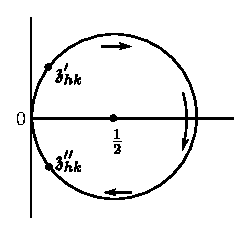
\includegraphics{vol2-figures/fig2.28.eps}}
\end{figure}
\end{minipage}
$$
\int\limits_{k^{(-)}} \Psi_k (\mathfrak{z}) e^{2 \pi n
  \mathfrak{z}/k^2} d\mathfrak{z}.
$$

This is an improper integral with both ends going to zero. That it
exists is clear, for what do we have to compensate for that? we have
to subtract $\int\limits_0^{\mathfrak{z}'_{hk}} \cdots$ and
$\int\limits^0_{\mathfrak{z}''_{hk}}\cdots$, and we prove that
these\pageoriginale\ indeed contribute very little. What is after all
$\Psi_k (\mathfrak{z})$?
$$
\Psi_k (\mathfrak{z}) = \sqrt{\mathfrak{z}} e^{\frac{\pi}{12}
  (\frac{1}{3} - \frac{\mathfrak{z}}{k^2})}
$$
$0< \mathscr{R} {\mathfrak{z}} \leq 1$ and $\mathscr{R}
1/\mathfrak{z}=1$ on the circle, so that
$$
\displaylines{\hfill |\Psi_k (\mathfrak{z})| \leq |\sqrt{\mathfrak{z}}
  e^{\pi/12}|\hfill \cr
\text{and} \hfill |e^{2 \pi n \mathfrak{z}/k^2}| \leq e^{2 \pi |n|};
\phantom{and}\hfill} 
$$
so that the integrand is bounded. Hence the limit exists. This is
indeed very astonishing, for $\Psi$ has an essential singularity at
the origin; but on the circle it does not do any harm. Near the origin
there are value which are as big as we want, but we can approach the
origin in a suitable way. This is the advantage of this contour. The
earlier treatment was very complicated.

\medskip
\noindent 
\begin{minipage}[c]{4.5cm}
  We can now estimate the integrals. Since $|\mathfrak{z}'_{hk}|\leq
  \surd 2 \cdot k/N$, the chord can be a little longer, in fact
  $\dfrac{\pi}{2}$ times the chord at most. So
\end{minipage}
\begin{minipage}[c]{5.5cm}
  \begin{figure}[H]
    \centering{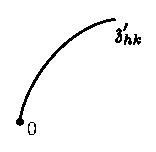
\includegraphics{vol2-figures/fig2.29.eps}}
  \end{figure}
\end{minipage}

\begin{align*}
  \left| \int\limits^{\mathfrak{z}'_{hk}}_0\right| & \leq \sqrt{2} \cdot
  \frac{\pi}{2} \frac{k}{N} e^{2 \pi |n|}
  \left(\frac{\surd\mathfrak{z} \cdot k}{N} \right)^{\frac{1}{2}}
  e^{\pi/12}\\
  & \leq C e^{2 \pi |n|} k^{3/2} N^{- 3/2}.
\end{align*}

The same estimate holds good for
$\int\limits^0_{\mathfrak{z}''_{hk}}\cdots$. Hence introducing. 

\begin{center}
  \LARGE{Page missing page No 165}\pageoriginale\
\end{center}

Now\pageoriginale\ everything is under our control. $N$ appeared
previously tacitly in $\mathfrak{z}'_{hk}$, because
$\mathfrak{z}'_{hk}$ depends on the Farey arc. Now $N$ appears in only
two places. So $p(n)$ is the limit of the sum which we write
symbolically as 
$$
p(n) = i \sum^\infty_{k=1} A_k (n) k^{-5/2} \int\limits_{K^{(-)}}
\Psi_k (\mathfrak{z}) e^{2 \pi n \mathfrak{z}/k^2} d\mathfrak{z}
$$
($n \gtreqless 0$, integral, and $p(n)=0$ for $n <0$). So we have an
exact infinite series for $p(n)$.

\medskip
\noindent 
\begin{minipage}[c]{4.5cm}
A thing of lesser significance is to determine the sum of this
series. So we have to speak about the integral. Let us take one more
step. Let us get away from the circle. Replace $z$ by
$\frac{1}{w}$. We do know what this will mean. $w$ will now run on a
line parallel to the imaginary axis, from $1- i \infty$ to $1+ i
\infty$. So
\end{minipage}
\begin{minipage}[c]{5.5cm}
  \begin{figure}[H]
    \centering{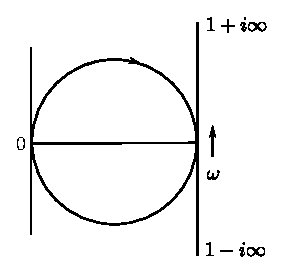
\includegraphics{vol2-figures/fig2.30.eps}}
  \end{figure}
\end{minipage}

\begin{align*}
  p(n) & = - \sum^\infty_{k=1} A_k (n) k^{-5/2} \int\limits^{1+ i
    \infty}_{1-i \infty} \omega^{- 1/2} e^{\frac{\pi}{12} (\omega -
    1/k^2 \omega)} e^{\frac{2 \pi n}{k^2 \omega}} \cdot \frac{d
    \omega}{\omega^2}\\
  & = \frac{1}{i} \sum^\infty_{k=1} A_k (n) k^{-5/12} \int\limits^{1+
    i \infty}_{1- i \infty} \omega^{- 5/2} e^{\frac{\pi}{2} +
    \frac{\pi}{12 k^2 \omega} (24n-1)} d \omega
\end{align*}

One\pageoriginale\ more step is advisable to get a little closer to
the customary notation. We then get traditional integrals known in
literature. Put $\dfrac{\pi \omega}{12}=s$,
$$
p(n) = \frac{1}{i} \left(\frac{\pi}{12} \right)^{3/2}
\sum^\infty_{k=1} A_k (n) k^{-5/2} \int\limits^{\frac{\pi}{12} + i
  \infty}_{\frac{\pi}{12} - i \infty} s^{-5/2} e^{s+
  \frac{\pi^2}{12k^{2s}}} (24n-1) ds
$$

One could look up Watson's `Bessel Functions' and write down this
integral as a Bessel function. But since we need the series anyway we
prefer to compute it directly. So we have to investigate an integral
of the type
$$
L(\nu) = \frac{1}{2 \pi i} \int\limits^{c+ i \infty}_{c- i \infty}
s^{- \nu-1} e^{s + \frac{\nu}{s}} ds
$$

It does not matter what $c>0$ is because it means only a shift to a
parallel line, and the integrand goes to zero for large imaginary part
of $s$. For absolute convergence it is enough to have a little more
than $s^{-1}$. So take $\mathscr{R} \nu >0$; in our case $\nu = 3/2$. 

So let us study the integral
$$
L_\nu (v) = \frac{1}{2 \pi i} \int\limits^{c+ i \infty}_{c- i
  \infty} s^{- \nu -1} e^{s+ \frac{v}{s}} ds
$$
  leaving it to the future what to do with $v$. The integration is
  along\pageoriginale\ a 

\medskip
\noindent
\begin{minipage}{4cm}
  line parallel to the imaginary axis. We now bend
  the path into a loop as in the figure and push the contour out, so
  that along the arcs we get negligible contributions. 
\end{minipage}
\begin{minipage}{6cm}
  \begin{figure}[H]
    \centering{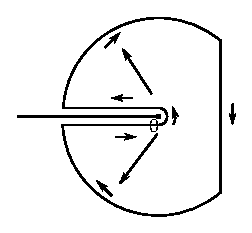
\includegraphics{vol2-figures/fig2.31.eps}}
  \end{figure}
\end{minipage}

The contribution from the arc $|s|=R$ is 
$$
O \left( \frac{1}{R^{\nu+1}\cdot R}\right)
$$
since $|e^{s + \frac{\nu}{s}}| \leq e^c e^{\mathscr{R} \nu/R}$, for a
fixed $v$; this is $O (R^{-\nu})\to 0$ as $R \to \infty$, since
$\nu >0$. So the integral along the ordinate becomes a `loop
integral', starting from $- \infty$ along the lower bank of the real
axis, looping around the origin and proceeding along the upper bank
towards $- \infty$; the loop integral is written in a fashion made
popular by Watson as
$$
\frac{1}{2 \pi i} \int\limits^{(0+)}_{- \infty} s^{-\nu -1} e^{s +
  \frac{\nu}{s}} ds
$$

For\pageoriginale\ better understanding we take a specific loop. On
the lower bank of the negative real axis we proceed only up to $-
\epsilon$, 
  \begin{figure}[H]
    \centering{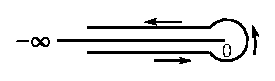
\includegraphics{vol2-figures/fig2.32.eps}}
  \end{figure}
then go round a circle of radius $\epsilon$ in the positive sense and
proceed thence along the upper bank, the integrand now having acquired
a new value-unless $\nu$ is an integer. This we take as a standardised
loop. We now prove that $L_\nu(\mathscr{V})$ is actually
differentiable and that the derivative can be obtained by
differentiating under the integral sign. For this we take $\left\{
L_\nu (\mathscr{V} +h) - L_\nu (\mathscr{V})\right\}/h$ and compare it
with what we could foresee to be $L'_{\nu} (\mathscr{V})$ and show
that the difference goes to zero as $h \to 0$.
\begin{multline*}
  \frac{L_\nu(\mathscr{V} +h)- L_\nu (\mathscr{V})}{h} - \frac{1}{2
    \pi i} \int\limits_{- \infty}^{(0+)} s^{- \nu-2} e^{s +
    \frac{\nu}{s}}ds\\  
  = \frac{1}{2 \pi i} \int\limits^{(0+)}_{-
    \infty} s^{- \nu -1} e^s \left\{ \frac{e^{\frac{v+h}{s} -
      e^{\frac{\nu}{s}}}}{h} - \frac{e^{\frac{\nu}{s}}}{s} \right\}
  ds\\
  = \frac{1}{2 \pi i} \int\limits^{(0+)}_{- \infty} s^{-
    \nu-1}e^{s+ \frac{\nu}{s}} \left\{ \frac{e^{\frac{h}{s}}-1}{h} -
  \frac{1}{s} \right\} ds
\end{multline*}

Now\pageoriginale\ 
\begin{align*}
  \frac{e^{\frac{h}{s}}-1}{h} - \frac{1}{s} & = \frac{\frac{h}{s} +
    \frac{h^2}{s^2 , s!} + \cdots}{h} - \frac{1}{s}\\
  & = h\left\{ \frac{1}{s^2\cdot 2!} + \frac{h}{s^3\cdot 3!} + \cdots
  \right\} 
\end{align*}

On the path of integration, $|s| \geq \epsilon > 0$; so
$$
\left| \frac{e^{\frac{h}{s}-1}}{h} - \frac{1}{s}\right|\leq C |h|,
$$
since we are having a quickly converging power series.
\begin{multline*}
  \therefore \quad \left| \frac{L_\nu (\nu +h)- L_\nu (\nu)}{h}-
  \frac{1}{2 \pi i} \int\limits^{(0+)}_{- \infty} s^{- v-2} e^{s+
    \frac{v}{s}} ds \right|\\
  \leq C|h| \left\{ 2 \int\limits^\infty_\epsilon \frac{1}{x^{v+1}} e^{-x}
  e^{\frac{\mathscr{R} \nu}{\epsilon}} dx + 2 \pi \epsilon \cdot
  \frac{1}{e^{\nu+1}} e^{\frac{\mathscr{R}\nu}{\epsilon}} \right\}  = 0(h) 
\end{multline*}

So the limit $\lim\limits_{h \to 0} \frac{L_v (\nu+h)- L_v(\nu)}{h}$
exists and $L_\nu (\nu)$ is differentiated uniformly in a circle of
any size. Since the differential integral is of the same shape we can
differentiate  under the integral as often as we please.

